\documentclass[12pt]{article}
\usepackage{float}
\usepackage{caption}
\usepackage{times}
\usepackage{natbib}
\usepackage{graphicx}
\usepackage[section]{placeins}
\usepackage{indentfirst}
\usepackage{fancyhdr}
\usepackage{xcolor}

\usepackage{listings}
\usepackage{color}
\usepackage[hyphens,spaces,obeyspaces]{url}
\usepackage{hyperref}
\pagenumbering{roman}
\hypersetup{
    colorlinks=true,
    linkcolor=blue,
    urlcolor=blue,
    citecolor = gray,
    linktoc=all
}

\pagestyle{fancy}
\fancyhf{}
\rhead{\textit{\color{gray}\today}}
\lhead{\textit{\color{gray}C++14 Software Transactional Memory}}
\rfoot{Page \thepage}
\lfoot{\color{gray}\LaTeX}

\pagenumbering{roman}
\begin{document}

\begin{titlepage}
	\begin{center}
	\line(1,0){350}\\
	[0.3 cm]
	\huge{\textbf{Software Transactional Memory\\[0.3 cm]C++14 STM\\ }} 
	\line(1,0){200}\\
	[0.3 cm]
	\huge{\textbf{Design manual }} 
		\begin{LARGE}
		\\[0.3 cm]Zoltan Fuzesi\\
		\today
		\end{LARGE}
		
		\begin{LARGE}
		\line(1,0){150}\\
		[1.0 cm]
		Student ID: C00197361\\
		Supervisor: Joseph Kehoe\\
		\color{gray}Institute of Technology Carlow\\
		\color{gray}Software Engineering
		\end{LARGE}
		
\begin{figure}[h!]
\centering

\includegraphics[scale=0.7]{Pictures/carlow.png}
\end{figure}
		
	\end{center}
\end{titlepage}

\tableofcontents







\clearpage
\pagenumbering{arabic}
\setcounter{page}{1}

\section{Introduction}
The document is introducing the design of the C++ STM library logic and structure. The document will describe the flow of the data within the library and the external application that uses the STM library. The use case diagram will discover the possible library API interface functionalities that need to implement in the project. With the use cases and the detailed use cases can characterize the required steps and potential alternative steps during the library execution life cycle. The domain model shows the main functionality of the library and the association between the software components, follows with the sequence diagram that helps to understand the sequence of steps required to follows each other to implement lock free atomic transaction.\\

This document helps to discover the potential errors and required handlers with the use cases and the sequence diagram. However, this diagrams and use case descriptions are identify the potential issues and risks, that may can mislead the future development if not well designed. To use or test the STM library implementation, the programmers must to write their own application and includes it like any external libraries in C or C++ programming design. The usage of the library can happen with the object method call that will be described in the use case diagram and studies thoroughly in the detailed use cases.\\
 
 
\newpage
\section{Model of the application}
The following flow diagram introducing the dynamic relationship of the STM library. This relations interacting with the external application and the objects delegated to the STM library. In order to use the STM library the programmers must include it, in the programmed module to create an instance to use the API interfaces. When the instances is created then the method call are available to the library object. The key of the library usage is that the programmers can not instantiate more then on object of the library per application, because the library will keep track of any single process involved in the transactional process by the process or thread ID in the library built in Data structure.

\subsection{Library integration to the application}
The library at compilation time get integrated into the C/C++ application. First the source code get transformed into intermediate code, that later get  compiled and linked with the STM library. As the STM library included in the source code, the library will be linked when the executable created from the application. \\

\begin{figure}[h!]
\centering
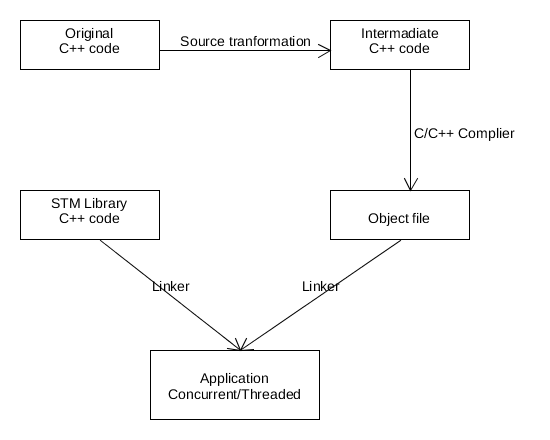
\includegraphics[scale=0.5]{Pictures/transformation.png}
\caption{\textit{\color{gray}STM library linked to application.}}
\end{figure}

\newpage
\subsection{Flow diagram}
\begin{figure}[h!]
\centering
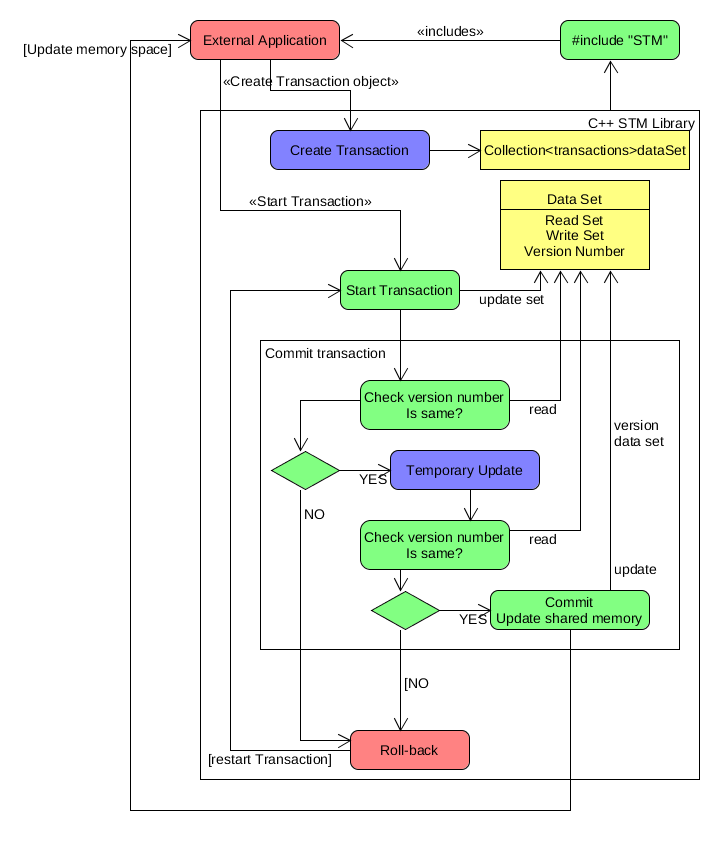
\includegraphics[scale=0.5]{Pictures/flowDiagram.png}
\caption{\textit{\color{gray}The flow of the data in the library.}}
\end{figure}

When the \textbf{create transaction} API call happens by the application, the library place the process into the built in data structure and returning back a transactional object.\\

The \textbf{start transaction} API call will starting the process of the Object transactional changes. Fist place the object into the read set and creates a copy of it to the write set to use it for local temporary changes, and a version number assigned to it as a counter for Object changes. Because more then one thread can use the same object it must check the version number at the first step to determine the changes at early stage of the transaction life cycle. If the version number in the object is different then the global version number the transaction will cancel and restart. if the transaction that the object hold and the global version number are same, then the copy of the object in the write set will update to the new required value. Before the original object can change from the local copy, the transaction library must check the version numbers equality. If the version numbers are same , that means no other process accessed the same object during the updating process and the object can get assign the new value. Otherwise, the transaction must cancel if the object has accessed by other process and the life cycle restart again.\\

In this phase of the program execution the transaction marked as processable process, and the \textbf{commit method} available for execution. This API call will update the original object, update the version number assigned to it and returns back to the main process and finish it execution. If other processes or thread are still using the same object, they must detect the changes on the version number, and restart the transactional if it required.

\section{Use case}
This section of the document the use case diagram will list the API actions or event steps, to define the interactions within the processes.

\begin{figure}[h!]
\centering
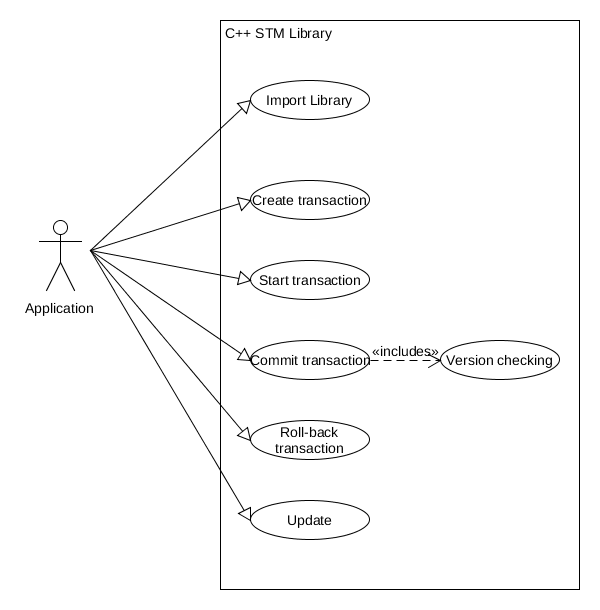
\includegraphics[scale=0.35]{Pictures/usacase.png}
\caption{\textit{\color{gray}The STM library API actions.}}
\end{figure}
{\setlength{\parindent}{0cm}
\subsection{Brief case}
\textbf{Use case} : Import library.\\
\textbf{Actors} : Application\\
\textbf{Description} : This use case begin when Application wants to use the STM library, then must include the library in the Application code from the host computer file system in order to able to instantiate an object of it later on in the Application, which ends this use case.\\

\textbf{Use case} : Create transaction.\\
\textbf{Actors} : Application\\
\textbf{Description} : This use case begin when Application wants instantiate an object of the STM transactional library. The library registering the process by the process/thread ID and returning a transactional object that can use the library API interface, which ends this use case.\\

\textbf{Use case} : Start transaction.\\\
\textbf{Actors} : Application\\
\textbf{Description} : This use case begin when Application wants to star  a new transactional process. The transactional object call the API function and send the Object which wants to operate on it. This object will be registered in the library read data set and a copy of it in the write data set, which ends this use case.\\  

\textbf{Use case} : Commit transaction.\\
\textbf{Actors} : Application\\
\textbf{Description} : This use case begin when Application wants commit or make permanent changes on the object shared value, while that is not available to the other processes. The transactional object calls the commit transaction function call. The library checking the version number associated with the object. If the version numbers are same in the global data set and the object itself the indicate the application that the object can be updated,  which ends this use case.\\ 

\textbf{Use case} : Roll-back transaction.\\
\textbf{Actors} : Application\\
\textbf{Description} : This use case begin when Application wants restart the transaction, because the commit function returned a false answer indicated the version umbers are not same. The roll back function will restart the process with the start transaction API call, which ends this use case. \\

\textbf{Use case} : Update transaction.\\
\textbf{Actors} : Application\\
\textbf{Description} : This use case begin when Application wants to update the object involved in the transaction. The transaction object calls the update API function, that will lock the object value of the other processes while updating. When the object value is updated, the library return a true value to the Application, which ends this use case.\\
}
\subsection{Detailed use case}
{\setlength{\parindent}{0cm}
\textbf{Name} : Create transaction.\\
\textbf{Actors} : Application\\
\textbf{Main Scenario.}
\begin{enumerate}
  \item The use case begins when the Application wants to create a transactional object.
  \item The Application passing the process/Thread and instantiate an object of the library.
  \item The library checks if the process in the data set.
  \item The library puts the process/Thread into the data set.
  \item The library returns the transactional object to the Application.
\end{enumerate}
\textbf{Alternatives}\\
4a. The library already registered the process and return the transaction object.\\

\textbf{Name} : Start transaction.\\
\textbf{Actors} : Application\\
\textbf{Main Scenario.}
\begin{enumerate}
  \item The use case begins when Application wants to make changes on an object value.
  \item The Application call the start transaction API function and passing the object to the library.
  \item The library registering the object to the read data set and creates  a copy of it to the write data set.
  \item The library assign a version number to the registered object.
  \item The library indicate the Application that the object registered.
\end{enumerate}
\textbf{Alternatives}\\
3a. The object already in the data set don't need to be register.\\

\textbf{Name} : Commit transaction.\\
\textbf{Actors} : Application\\
\textbf{Main Scenario.}
\begin{enumerate}
  \item The use case begins when the Application wants to make the changes on the object value.
  \item The Application calls the commit transaction function call on the API and passing the required values to exchange within the object.
  \item The library checks the version number associated with the object.
  \item The library make changes on the copy of the object in the local data set.
  \item The library checks again the version number associated with the object. 
  \item The library indicates the Application that the changes has made and ready to update.
\end{enumerate}
\textbf{Alternatives}\\
3a. The library early find the difference between the version numbers.\\
3b. The library cancel the transaction and indicates the Application with a false answer.\\
5a. The library later stage find the difference between the version numbers.\\
5b. The library cancel the transaction and indicates the Application with a false answer.\\


\textbf{Name} : Roll-back transaction.\\
\textbf{Actors} : Application\\
\textbf{Main Scenario.}
\begin{enumerate}
  \item The use case begins when the Application wants to roll back the transaction.
  \item The Application after receive a false answer from the library of the commit transaction will call the roll back API function call.
  \item The library rolling back the changes on the copy of the object in the local data set.
  \item The library restart the transaction. 
\end{enumerate}


\textbf{Name} : Update transaction.\\
\textbf{Actors} : Application\\
\textbf{Main Scenario.}
\begin{enumerate}
  \item The use case begins when the Application wants to update the value on the object value.
  \item The Application calls the update transaction function in the library API.
  \item The library locks the shared memory space in front of the other processes.
  \item The library update the object from the local data set.
  \item The library release the lock and increase the version number associated with the object.
  \item The library indicates the Application that the changes has made.
\end{enumerate}

}

\newpage
\section{Domain model}
The domain model is quiet simple since the library do not need include many classes and functions to implement the Software Transactional Memory implementation with the basic functions. Of course, many STM library has implementation of different binary trees as well, that make it more bigger and complex. 
\begin{figure}[h!]
\centering
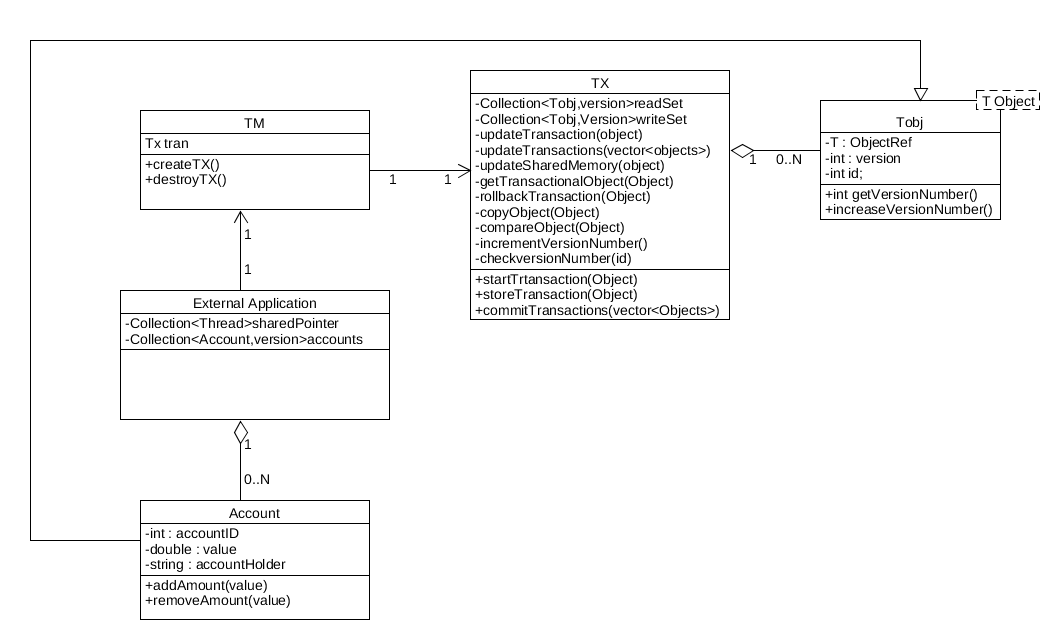
\includegraphics[scale=0.5]{Pictures/domainModel.png}
\caption{\textit{\color{gray}The class hierarchy.}}
\end{figure}

\newpage
\section{System sequence diagram}
\begin{figure}[h!]
\centering
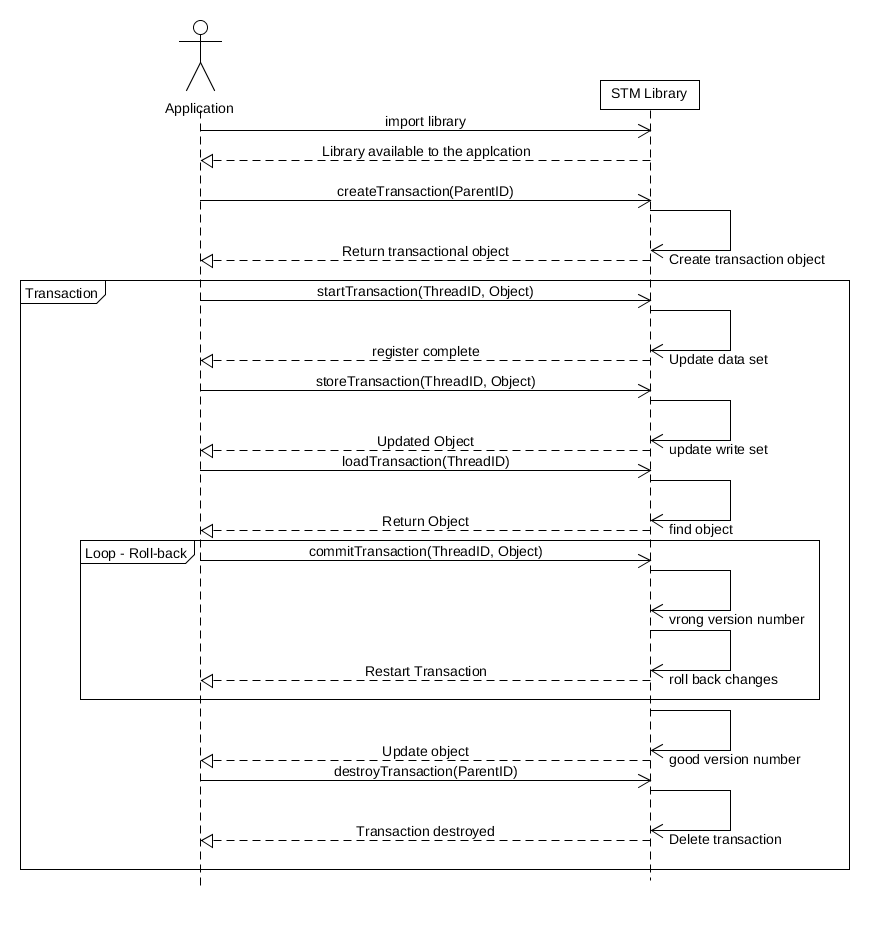
\includegraphics[scale=0.5]{Pictures/sequence.png}
\caption{\textit{\color{gray}The system sequence diagram.}}
\end{figure}

\newpage
\section{Testing the STM Library}
The only way to test the Software Transaction Memory library functionalities, is to create an application and include the shared library in it. Test is a very important process of the project life cycle.
As the library getting more functionality during the development, those functions should be tested one by one. Because the functions have return values, it makes the testing process more easier.\\

\textbf{The functions can be tested separately like:}
\begin{enumerate}
\item The library available from the test application.
\item The library can be instantiated by the application.
\item The instance of the library object can access the API function.
\item The functions are working properly as they are expected.
\item The library can lock the shared variable in front of the other processes.
\item The library able to detect the version conflicts during the transaction.
\item The library returns the correct values after the transactions.
\end{enumerate}


The library should able to handle single or multiple threaded environments as well.



\section{Conclusion}
The design document helps to discover the functionality and the association between system components. Give a clearer picture of the project functions, sequence of the processes and relation between the application and the library.\\

Because this project developed in an Agile way, the described functions and system components my will change during the future development in the project life cycle.


\end{document}